\documentclass[10pt]{beamer}
\usefonttheme{professionalfonts}
%\usetheme{CambridgeUS}
%
% Choose how your presentation looks.
%
% For more themes, color themes and font themes, see:
% http://deic.uab.es/~iblanes/beamer_gallery/index_by_theme.html
%
\mode<presentation>
{
  \usetheme{default}      % or try Darmstadt, Madrid, Warsaw, ...
  \usecolortheme{beaver} % or try albatross, beaver, crane, ...
  \usefonttheme{default}  % or try serif, structurebold, ...
  \setbeamertemplate{navigation symbols}{}
  \setbeamertemplate{caption}[numbered]
} 

\usepackage[english]{babel}
\usepackage[utf8x]{inputenc}
\usepackage{tikz}
\usepackage{pgfplots}
\usepackage{array}  % for table column M
\usepackage{makecell} % to break line within a cell
\usepackage{verbatim}
\usepackage{graphicx}
\usepackage{epstopdf}
\usepackage{amsfonts}
\usepackage{xcolor}
\usepackage{ifthen}
\usepackage[makeroom]{cancel}
%\captionsetup{compatibility=false}
%\usepackage{dsfont}
\usepackage[absolute,overlay]{textpos}
\usetikzlibrary{calc, angles,quotes}
\usetikzlibrary{pgfplots.fillbetween, backgrounds}
\usetikzlibrary{positioning}
\usetikzlibrary{arrows}
\usetikzlibrary{pgfplots.groupplots}
\usetikzlibrary{arrows.meta}
\usetikzlibrary{plotmarks}
\usetikzlibrary{decorations.markings}

\usepgfplotslibrary{groupplots}
\pgfplotsset{compat=newest} 

\definecolor{blue2}{RGB}{51, 105, 232}  
\definecolor{red2}{RGB}{213, 15, 37}  
\definecolor{green2}{RGB}{0, 153, 37}  
\definecolor{green3}{rgb}{0.1922, 0.6392, 0.3294}% 
\definecolor{yellow2}{RGB}{238, 178, 17} 
\definecolor{gray2}{RGB}{102, 102, 102}
\definecolor{orange2}{RGB}{230, 85, 13}

% Qualitative pallete set1 from www.ColorBrewer.org
\definecolor{Qred}{RGB}{228,26,28}
\definecolor{Qblue}{RGB}{55,126,184}
\definecolor{Qgreen}{RGB}{77,175,74}
\definecolor{Qpurple}{RGB}{152,78,163}
\definecolor{Qorange}{RGB}{255,127,0}
\definecolor{Qyellow}{RGB}{255,255,51}
\definecolor{Qbrown}{RGB}{166,86,40}
\definecolor{Qpink}{RGB}{247,129,191}
\definecolor{Qgray}{RGB}{153,153,153}

\begin{document}
	\begin{frame}
	\centering
	\resizebox{\textwidth}{!}{
	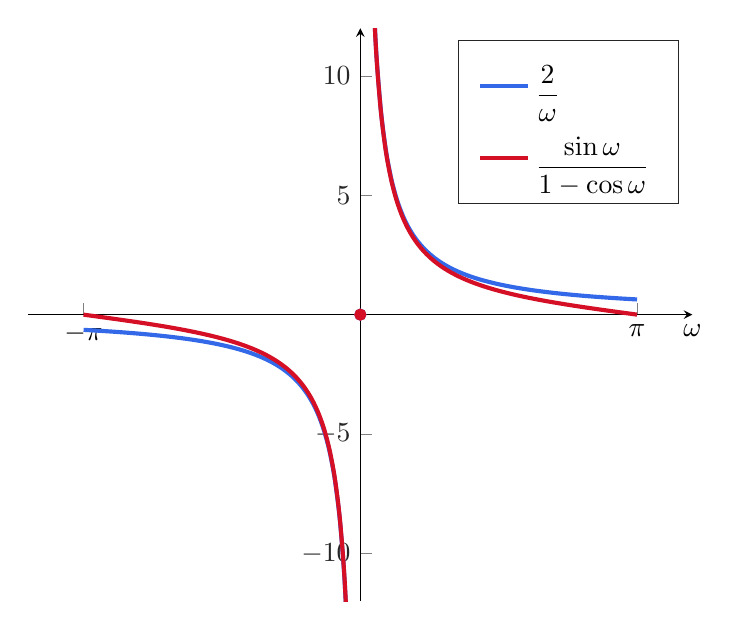
\begin{tikzpicture}
		\begin{axis}[
		name=plot1,
		axis lines*=middle,
		enlargelimits = true,
		clip=true,
		scale only axis,
		ymin=-10,	ymax=10,
		xmin=-3.14, xmax=3.14,
		axis line style={->,>=stealth},
		xlabel={$\omega$},
		%ylabel={\small $X(e^{j\omega})$},
		every axis x label/.style={
			at={(ticklabel* cs:1)},
			%xshift=0.2cm,
			anchor=north,
		},
		every axis y label/.style={
			at={(ticklabel* cs:0.8)},
			anchor=south,
			xshift=0.6cm,
		},
		xtick={-3.14, 3.14},
		xticklabels={$-\pi$, $\pi$}, 
		every outer y axis line/.append style={white!15!black},
		every y tick label/.append style={font=\color{white!15!black}},
		legend style={draw=white!15!black,fill=white,legend cell align=left, text width=1.5cm, row sep=0.25cm, inner sep=0.25cm}]
			\addplot[smooth, blue2, solid, line width = 1.5pt, domain=0.1:3.14, samples=50] {2/x}; \addlegendentry{$\displaystyle\frac{2}{\omega}$};
			\addplot[smooth, red2, solid, line width = 1.5pt, domain=0.1:3.14, samples=50] {sin(deg(x))/(1-cos(deg(x))}; \addlegendentry{$\displaystyle\frac{\sin\omega}{1-\cos\omega}$};
			
			\addplot[smooth, blue2, solid, line width = 1.5pt, domain=-3.14:-0.1, samples=50, forget plot] {2/x};
			\addplot[smooth, red2, solid, line width = 1.5pt, domain=-3.14:-0.1, samples=50] {sin(deg(x))/(1-cos(deg(x))};
			
			\addplot[mark=*, blue2, mark size=2pt, forget plot] coordinates {(0, 0)};
			\addplot[mark=*, red2, mark size=2pt, forget plot] coordinates {(0, 0)};
		\end{axis}
		\end{tikzpicture}
	}
	\end{frame}
\end{document}